%% Quick build: [path]/convert.sh|pdflatex -synctex=1 -interaction=nonstopmode %.tex|biber %.bcf|pdflatex -synctex=1 -interaction=nonstopmode %.tex|pdflatex -synctex=1 -interaction=nonstopmode %.tex|evince %.pdf

\documentclass[doc]{apa6}
\usepackage[utf8]{inputenc}
\usepackage[english]{babel}
\usepackage{csquotes}
\usepackage[style=apa,sortcites=true,sorting=nyt,backend=biber]{biblatex}

\usepackage{amsmath}
\usepackage{amsfonts}
\usepackage{amssymb}
\usepackage{gensymb}
\usepackage[load=abbr]{siunitx}
\usepackage{setspace}	% for line spacing
\usepackage{calc}		% for figure scaling
\usepackage{svg}		% for graphics
\usepackage{graphicx}	% for graphics
\usepackage[left=1in,right=1in,top=1in,bottom=1in]{geometry}
\usepackage{listings}
\usepackage{minted}
\usepackage{subcaption}
\usepackage{wrapfig}

\lstset{language = Python, basicstyle = \small\ttfamily, tabsize = 4}

%\DeclareLanguageMapping{american}{american-apa}
\addbibresource{/home/rob/Documents/bibtex/library.bib}

\linespread{1.5}

% Images are build by calling images/generate.sh <images> <output> where
% output is the "build" directory used by Texmaker.
\graphicspath{{./build/images/}}

\DeclareUnicodeCharacter{2010}{ }

%\lstset{%
%  basicstyle=\small\ttfamily,
%  language=Python
%}


\shorttitle{}

\title{Proposed Method for Using Cubic Splines for the Control of Remote-Sensing Unmanned Aerial Vehicles}
\author{Rob Skelly}
\affiliation{University of Victoria}
\note{Geography 599, Spring 2019}

%\abstract{}

\begin{document}

\maketitle



\section{Introduction}

In the field of remote sensing with unmanned aerial vehicles (UAVs), the maintenance of data quality is can be managed, in part, by stabilising the instrument-to-subject distance and orientation. This can be accomplished by controlling the vehicle's altitude and attitude, respectively.

UAV surveys are generally pre-planned using purpose-built software and followed (semi-)automonmously by the aircraft. Most currently-available software allows the creation of flight plans only in the horizontal plane \parencite[e.g.,][]{ArduPilot2018,DJI2018a,Microdrones2018,Group2018,UAVToolbox2018}, leaving it to the pilot to set a constant -- usually barometric -- altitude sufficient to clear the terrain and any obstacles in the study area. Those packages that do enable terrain avoidance rely on an  existing digital elevation model (DEM) \parencite[e.g.,][]{PrecisionHawk2018,UgCS2018,MapsMadeEasy2018}, or use a nadir-aligned rangefinder for \emph{reactive} terrain avoidance.

In the remote sensing context, \emph{terrain avoidance} is distinct from \emph{surface following}: the objective is not merely to avoid colliding with the terrain, but to maintain an altitude and attitude with respect to the sensed surface (which may be a vegetative canopy or the terrain itself) which preserves the quality -- image scale and distortion, point density, signal-to-noise ratio, swath overlap, etc. -- of the data products. Given limitations on the energy-density of current batteries, and thus flight duration, the ability to follow a trajectory safely and efficiently is also a major concern.

This research pursues the development of a real-time, predictive flight-planning system for UAV remote sensing, to satisfy the data-quality objectives of a remote-sensing mission while resolving some of the inadequacies of existing mission-planning software packages. The system will use a forward-looking laser rangefinder to generate a two-dimensional point cloud from which a trajectory, a cubic spline, will be computed.

Specifically, this proposal outlines a rationale and methodology for selecting the type of piecwise cubic spline (e.g., interpolating, smoothing, natural, constrained, weighted) to represent the trajectory, whose characteristics best satisfy the data-quality, efficiency and safety constraints as described. 



\section{Background}

\subsection{UAV Remote Sensing}

Unmanned aerial vehicles (UAVs) are small reusable aircraft, controlled remotely by a human operator or (semi-)autonomously, which can range in size from insect-scale to jet-powered military aircraft \parencite{Avadhanula2002,Deng2003} and are subject to an ongoing explosion in engineering, scientific, military and commercial interest. 

In the scientific remote-sensing field, where the execution of an aerial survey could entail hundreds of thousands of dollars in costs for planning, permitting, instrumentation, pilots and aircraft, the advent of UAVs provides researchers with the opportunity to conduct research at much lower cost with little turnaround time. 

Traditional aerial surveys have the advantage that, at typical survey altitudes of $\SI{250}\m-\SI{1000}\m$, variations in terrain relief and vegetation canopy height (collectively, surface height) are insignificant relative to the platform altitude -- except in extreme cases, such as alpine terrain -- causing minimal scale distortion in the resulting imagery. Low-altitude UAV surveys, which may take place at $\SI{10}\m-\SI{50}\m$ above the surface, encounter much larger relative variations in surface height and so must follow the surface, both to maintain the subject distance and to avoid colliding with it. In addition, because there are many structures, both natural and human-made, that may project above a UAV's trajectory, the vehicle must have the ability to detect and avoid hazards. Manned aircraft, with an alert pilot and high altitude, rarely face such obstacles. 


\subsection{Data Quality}

The quality of remotely-sensed data can be quantified in a number of ways. Variation in the average posting distance, or point density, of a LiDAR point cloud affects the power of any statistical derivatives and fluctuations in atmospheric attenuation, path radiance, scale and signal-to-noise ratio affect the quality of spectrometry. These are attributable to the platform velocity, altitude and attitude which, as the instruments are fixed to the airframe, must be carefully maintained by the flight controller. In general, the lower the nominal altitude, for a given site, the larger the effect of surface height variation on data quality. For examle, at $\SI{10}\m$ nominal flight altitude, a variation of $\pm\SI{2}\m$ induces a variation in image scale of $\%40$.  

A final important aspect of data quality is time-of-collection. A spectral survey is ideally conducted as near as possible to solar noon under stable atmospheric conditions. A researcher must be opportunistic and maximise productivity during this time. In general, remote sensing surveys using UAVs cannot be conducted in high winds, outside of dailight hours or during precipitation events. Repeating a survey to produce a DEM or terrain following, or interrupting one to change batteries, may delay the completion of the survey or limit the size of the study site, and splitting the survey over multiple days risks not only a change in the weather, but a an advance in the state of whatever phenomenon is under observation. 


\subsection{Surface Following}

The foregoing quality and efficiency concerns can be resolved, at least in part, by a real-time surface-following system that accurately maintains the altitude of the aircraft above the surface while minimising disturbances to its attitude and velocity. 

Reactive systems using nadir-aligned rangefinders, cannot anticipate variations surface height and so have no way of forecasting a trajectory that protects data quality while repsecting the dynamic limitations of the aircraft.

Mission planning packages that allow the selection or production of a digital elevation model (DEM) \parencite[e.g.,][]{PrecisionHawk2018,UgCS2018,MapsMadeEasy2018}, are either tied to coarse, publicly-available datasets, such as the Shuttle Radar Topography Mission (SRTM), or require a pre-flight and subsequent photogrammetric or LiDAR processing to produce a DEM. 

Publicly-available DEMs may be out of date, poorly-documented, incompatible with the working coordinate system and datum or of doubtful provenance. The SRTM mission in particular used C- and X-band radar, which penetrates a vegetative canopy to a variable degree depending on the type of vegetaion, density, gap structure, senescence, wetness and other factors \parencite{Miliaresis2009}, significantly underestimating their height \parencite{Sexton2009}. As well, the SRTM represents the surface of the Earth, at the time of writing, 19 years in the past. 

If a DEM must be produced in the field, a preliminary survey is required, meaning that at least two full surveys must be conducted, plus the processing time required to produce the model. Since the model must be produced first, the researcher has no way of knowing if conditions will still be suitable by the time the second survey begins. In any case, such a strategy essentially doubles the total amount of work, cost and risk of any survey. 

A real-time, predictive surface-following system obviates the need for these additional flights, allowing the researcher to conduct surveys during ideal conditions as they arise, and to adapt the flight plan in the field as necessary.

Any surface-following system must be able to accomodate the different surface charactistics and mission objectives that a researcher may encounter. For example, a vineyard's rows (figure \ref{fig:photo_culmina_rows}) are spaced approximately $\SI{2}\m$ apart, leaving a depression between the rows. It would be undesireable for the aircraft to descend into each depression; rather, its trajectory should carry it smoothly over a surface implied by the tops of the rows while it follows the low-frequency variations in the terrain (fgure \ref{fig:photo_culmina_rows_slope}). (On the other hand, if the researcher were interested in imaging the sides of each vine as well as the tops, following this high-frequency surface variation would be desirable.) In this sense, a surface-following system is a low-pass filter with configurable sensitivity. 

\begin{figure} %[htbp] % htbp stand for "here", "top", "bottom", "page"
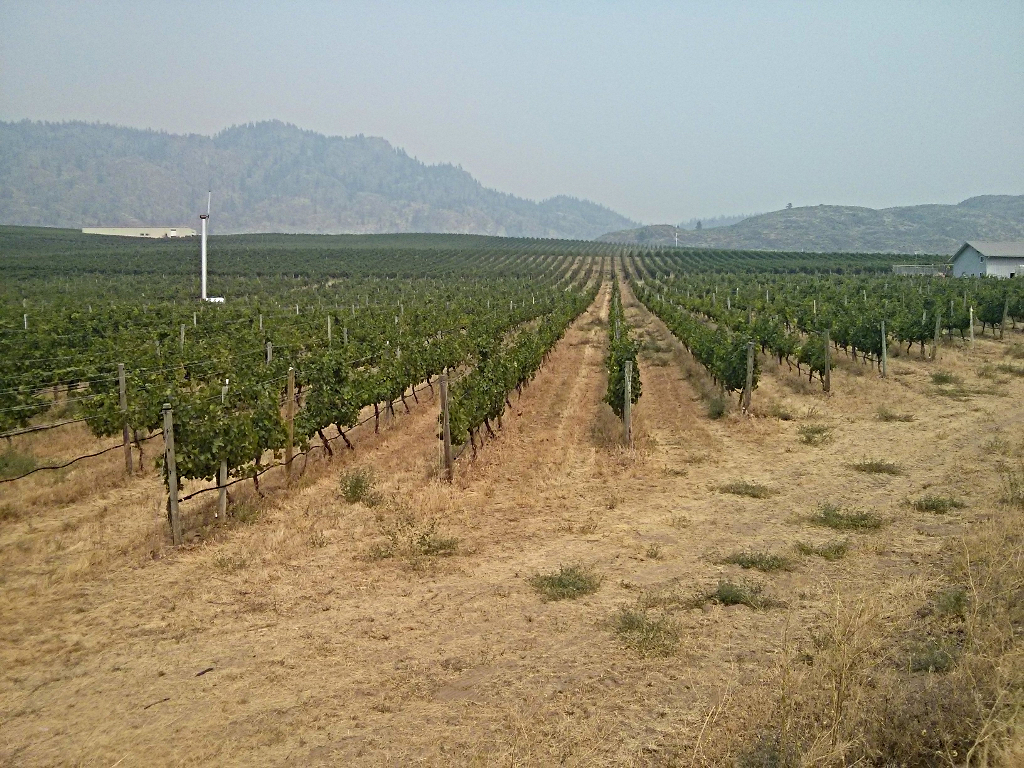
\includegraphics[width=1.0\linewidth]{tmp/photo_culmina_rows.pdf} 
\caption{Typical spacing of vinyard rows. Culmina Winery, Penticton, BC. August 2017.}
\label{fig:photo_culmina_rows}
\end{figure}

\begin{figure} %[htbp] % htbp stand for "here", "top", "bottom", "page"
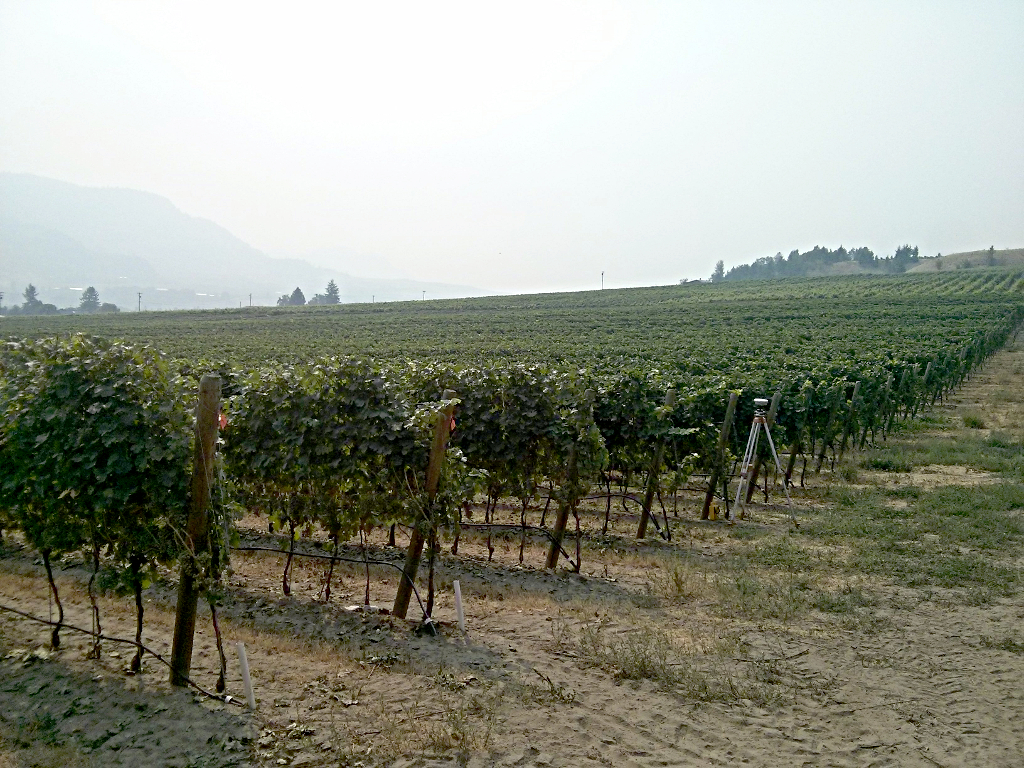
\includegraphics[width=1.0\linewidth]{tmp/photo_culmina_rows_slope.pdf} 
\caption{Low-frequency surface height variation, Culmina Winery, Penticton, BC. August 2017.}
\label{fig:photo_culmina_rows_slope}
\end{figure}


\subsection{Splines}

If it is desireable to quantify the constraints on a trajectory -- to minimize power consumption and deviation of the trajectory with respect to the imaged surface -- then it is desireable to produce a trajectory that is representable as a smooth, differentiable function. First, because the physical body of the aircraft must obey certain dynamic laws which are easily representable by the derivatives of such a function; second, because the fidelity of the function can be measured at any location. The cubic spline is a promising candidate.

\begin{figure} %[htbp] % htbp stand for "here", "top", "bottom", "page"
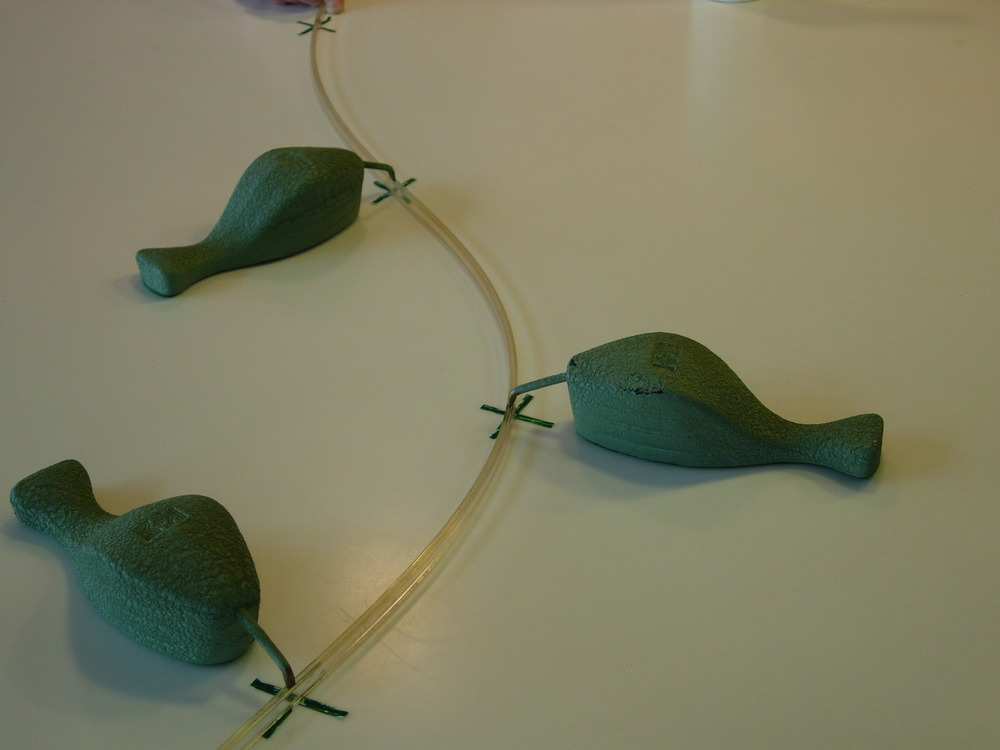
\includegraphics[width=1.0\linewidth]{tmp/draftspline.pdf} 
\caption{A draftsman's spline and ``ducks.'' \parencite{DeBoor2006}}
\label{fig:spline}
\end{figure}

The word ``spline'' originates in drafting, where long, flexible wooden or plastic beams, called splines (figure \ref{fig:spline}), were used to model curves. A spline would be placed on the drawing, held down by two or more lead weights called ``ducks,'' and would seek a shape which minimized the energy stored in the beam. The spline could thus be considered an optimal interpolator \parencite{Wegman2016}. 

In mathematics, the spline is consists of a set of piecewise (usually cubic) polynomials, one each between each pair of ducks, or ``knots.'' At each knot, the zeroth, first, and possibly higher, derivatives of the adjoining polynomials are held equal, resulting an a curve that is smooth and differentiable along its entire length. The minimum-energy constraint is modelled by minimizing mean square curvature of the polynomial \parencite{Wegman2016}.

In this instance, the spline function is used to model the behaviour of a physical body in space, with velocity and acceleration given by the first and second derivatives, respectively. The second derivative is of particular interest because it is constrained by the aircraft's dynamic properties given by Newton's second law,

\begin{equation}
F = ma,
\end{equation} 

where $F$ is force, in Newtons, $m$ is the mass of the vehicle in kg, and $a$ is the acceleration in $m/s$. Forces on the airframe are generated by the propulsion system, gravity and aerodynamic drag. When the second derivative is positive, its magnitude can be no greater than the acceleration provided by the net of these forces (climbing under maximum thrust). When negative, its magnitude can be no greater than net of these forces with thrust set to near zero (freefall). These constraints may be derived from the aircraft's thrust, as documented by the manufacturer, and its mass and air resistance, which must be measured. The maximum vertical velocity -- the second derivative -- of most UAVs is documented by the manufacturer and limited by the flight controller. Whether the vehicle can acheive the velocity limit depends on its mass (including cargo) and the force supplied by its propulsion system.

Though cubic splines are smooth and twice differentiable, it will be observed that the second derivative (acceleration) is not smooth, having cusps at the knots (figure \ref{fig:cubic_derivatives}.) For any polynomial, for some value of $m > 0$, the $m$th derivative will be linear; for cubic splines, this occurs at $m = 2$. This is not a concern, so long as the change of thrust by the aircraft's flight controller is assumed to occur instantaneously. It does not, of course, as it takes time to supply the motors with power, and for their rotational velocity to change. Here, the maximum thrust, or some multiple less than $1$ will be used as an estimate of the limit.

The mechanical spline and its mathematical equivalent are interpolators and pass through each of the knots. If the knots of the spline are close together, or form a steep gradient, un-resolvable loops or overshoots could form in the spline, resulting in a physically-impossible trajectory. A variation on the interpolating spline, the weighted spline, allows the calculation of a weight, applied at each knot, which can suppress the tendency for overshoots \parencite{lancaster1986curve}. However this breaks the continuity of the second derivative, which in turn breaks the physical model.


\subsection{Smoothing Splines}

An alternative construction -- the smoothing or approximating spline -- allows the spline to preserve the overall shape of the data distribution -- that is, the measured surface -- without passing through each knot exactly.

A smoothing spline has two conflicting objectives \parencite{lancaster1986curve, Drakos2002, Boor2001, Reinsch1967}:
\begin{enumerate}
\item To minimize the sum of squared distances between the function estimate and the ordinates;
\item To minimize the curvature of the function.
\end{enumerate}

This leads to de Boor's formulation,

\begin{equation}
S(x) = p \sum_{i=1}^{n} \left( {(Y_i - \hat{f}(x_i))^2 \over {\sigma_i}^2} \right) + (1 - p) \int{ \left( \hat{f}^{(m)}(x) \right)^2 } dx,
\end{equation}

where the first term is essentialy a Chi-square measure of the data distribution and the second a measure of its curvature, both weighted by $p \in{[0-1]}$ or its negation. Here, $Y$ is the ordinate, $\hat{f}$ is the spline estimate and $\sigma$ represents the variance of the ordinate set. $p$ has the effect of controlling the number of knots: as $p$ approaches $1$, the first term is emphasized, forcing a closer fit to the data, while as $p$ approaces $0$, the integral is emphasized, forcing a straighter (smoother) curve. As the fit improves, the number of knots and their positions approach those of the oridinates; as smoothness increases, a straight line emerges with two knots at the ends.

The system is constrained, such that,

\begin{equation}
\begin{split}
S(x_{i-1}) &= S(x_i), \\
S'(x_{i-1}) &= S'(x_i), and \\ 
S''(x_{i-1}) &= S''(x_i).
\end{split}
\end{equation}

At each knot, the ends of adjoining splines have not only the same value, but the same first (slope) and second (curvature) derivatives. In this usage, the function value is the vehicle altitude with the first and second derivatives representing velocity and acceleration, respectively. To find the spline function, it is possible by indefinite integration to find the original function, beginning with the slopes at the end of the segment and two knots. In the case of the so-called ``natural spline'', the second derivatives at the first and last knots are held to zero. 

Figure \ref{fig:cubic_derivatives} shows a preliminary study of the cubic smoothing spline and derivatives computed on a real-world LiDAR point cloud, using the concave hull ($\alpha = 10m$) for surface-point extraction.

\begin{figure} %[htbp] % htbp stand for "here", "top", "bottom", "page"
\includegraphics[width=1.0\linewidth]{tmp/splines_derivs_smooth_0_5_weight_0_1.pdf} 
\caption{Smoothing cubic spline through the vertices of concave hull derived from a real-world point cloud. First and second derivatives correspond velocity and acceleration, assuming horizontal velocity of 1m/s.}
\label{fig:cubic_derivatives}
\end{figure}

It is evident that the smoothing spline is a good candidate for examination as a trajectory function, as its derivatives provide a means of modeling the physical dynamics of the vehicle and it can be adjusted to satisfy the dynamic and data-quality constraints. The ability to interpret the general shape of a surface without interpolating all points exactly -- which would result in deleterious, difficult-to-resolve artifacts -- is a boon.

What remains is to develop a methodology for selecting weight and smoothness parameters appropriate to these constraints, given the available instrumentation and computational resources.


\section{Methods}

The input to the process described in this study is a sorted (in the y-dimension) two-dimensional (planar) point cloud, oriented in the y-z axis of the aircaft, that is, vertical and fore-aft. This point cloud is generated by a forward-facing scanning laser rangefinder, and the x-dimension collapsed. For this study, the point cloud is simulated by selecting points within a selected distance of a hyperplane with the aircraft position as its origin and the normal in the x-axis. 

The output is a set of parameterized splines that the vehicle will use to set its altitude as it flies.

There is a difficulty with the UAV use-case: the point cloud is never complete at any time during the flight, so the trajectory must be computed piece-wise in real-time as sufficient data is obtained. Once a trajectory is computed it must not be altered by newly-arrived data, lest discontinuities appear in the trajectory as its position changes. One way to overcome this difficulty might be to compute the spline over ``blocks'' of point cloud. When a block is deemed complete, it is considered ``finalized'' and the trajectory extracted from it. If the spline is computed with the ``natural'' constraint ($S''(x_0) = S''(n) = 0$) then the vehicle's throttle setting can be assumed to remain constant accross each block boundary. It remains to determine whether enough points can be collected, finalized and processed for each block in time to provide useful trajectory information to the vehicle before it crosses the next boundary.

As this issue remains unresolved, this paper focuses on the development and analysis of a trajectory derived from an entire, intact point cloud.


\subsection{Surface Reconstruction}

Some representation of the imaged ``surface'' must be extracted from the point cloud. If this were not done, points from the interior of the vegetative canopy or the terrain would bias the spline downward, degrading the data quality and possibly precipitating a crash. The point subset must contain enough points to provide some surface detail and few enough to obscure high-frequency variation and ensure efficient computability. 

However, the definition of a ``surface'' is problematic. The points represent measurements of real objects but provide no information about what exists between those objects. The surface is fractal \parencite{Mandelbrot1967}.

One conception of the surface is that one's  certainty about its height is perfect at the location of a point, A, and degrades with distance from that point. As this distance increases the distance to a neighbouring point, B, decreases, and one's certainty about the height of the surface relative to B increases. (This premise, Tobler's law \parencite{Tobler1970a}, is fundamental to quantitative geography.) The point cloud thus implies probabilistic, interpolating surface. 

A simple, efficient way of extracting an interpolating surface from a 2-dimensional point cloud is to compute the convex hull. Unfortunately, on surfaces that have anything other than a convex, or domed, shape, most of the surface detail is lost. Alternatively, a \emph{concave} hull would allow for indents in the surface. Unlike the convex hull -- the unique minimum polygon containing the all constituent hulls of the point-set -- there is no single definition of a concave hull. Alpha shapes \parencite{Edelsbrunner1994} are a well-defined candidate, but require the triangulation (via Delaunay) of the entire point set. Another alternative is to modify an existing fast convex hull algorithm to limit the maximum segment length.

\begin{figure} %[htbp] % htbp stand for "here", "top", "bottom", "page"
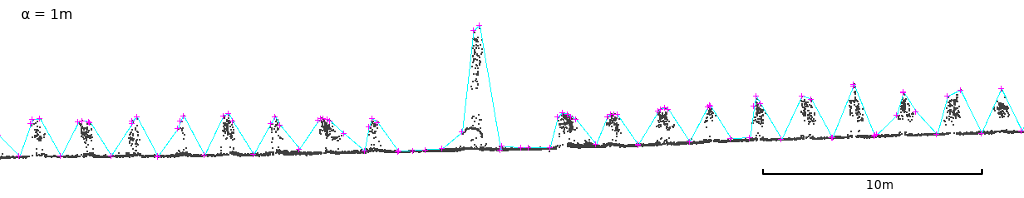
\includegraphics[width=1.0\linewidth]{tmp/concave_1.pdf} 
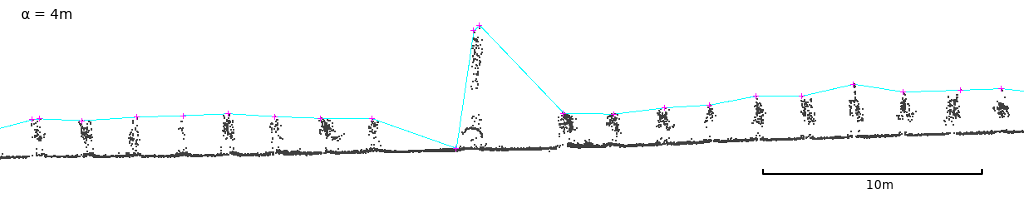
\includegraphics[width=1.0\linewidth]{tmp/concave_4.pdf} 
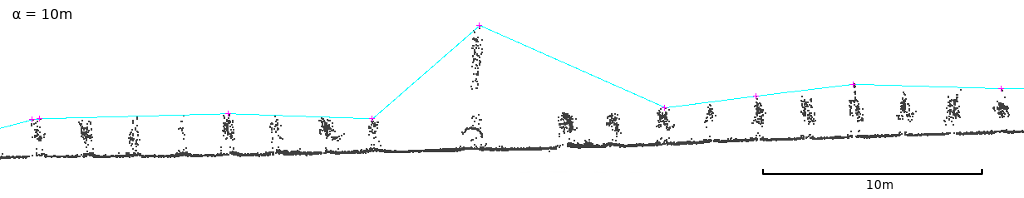
\includegraphics[width=1.0\linewidth]{tmp/concave_10.pdf} 
\caption{Concave hull surface extraction using three $\alpha$ values: $\SI{1}\m$, $\SI{4}\m$ and $\SI{10}\m$. Grey points represent the original point cloud, the cyan line is the hull and fuscha crosses represent vertices. The tradeoff between point count and surface detail is evident.}
\label{fig:concave}
\end{figure}

The Mototone Chain convex hull algorithm \parencite{Andrew1979} runs in linear ($O(n)$) time, in constant space, on a sorted point set, which is the expected state of the input. By modifying the main loop of the algorithm to limit the length of any given segment (via a parameter, $\alpha$) and running it only on the upper surface of the input, it becomes a configurable surface-extraction tool. 

However, though the maximum segment length can be enforced, there can be no minimum. This leads to possible clustering of vertices near highly curved sections of the surface. The method is also asymmetrical: the result in one direction will differ from the result in the opposite direction. In concrete terms, this means that, when a depression is encountered, a maximum-length segment will reach across the depression to the opposite side, then a cluster of vertices will occur as the algorithm ``climbs'' the convex slope of the far side.

The vertices of the concave hull form the point-set upon which the trajectory is computed. In general, a larger $\alpha$ value results in a larger number of vertices. A Python implementation of the concave hull algorithm is given in Listing \ref{lst:concave_hull}. 

\begin{listing}
\begin{minted}{python}

def hull(pts, alpha):

	hull = pts[:2]

	for i in range(2, len(pts)):
	
		while len(hull) >= 2 
				and cross(hull[-2], hull[-1], pts[i]) >= 0 
				and lengthY(hull[-2], pts[i]) <= alpha ** 2:

			hull.pop()

		hull.append(pts[i])

	return hull

\end{minted}
\caption{Modified Monotone Chain algorithm for constructing a convex hull. The \lstinline{cross} function determines whether the segment makes a clockwise or counterclockwise turn; \lstinline{lengthY} gives the distance between points in $y$. The \lstinline{pts} array is a list of points, sorted on $y$; \lstinline{alpha} is the maximum segment length.}
\label{lst:concave_hull}
\end{listing}

\begin{wrapfigure}{r}{0.5\textwidth} %[htbp] % htbp stand for "here", "top", "bottom", "page"
\begin{center}
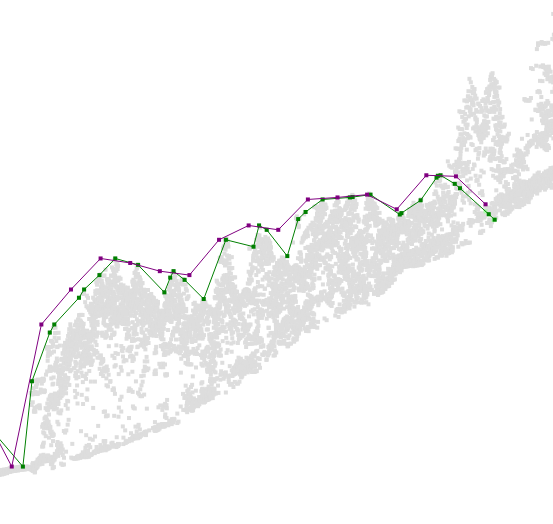
\includegraphics[width=0.45\textwidth]{tmp/hull_vs_bin.pdf} 
\end{center}
\caption{Comparison of concave hull (green) and binning (purple) surface extraction.}
\label{fig:bin_vs_hull}
\end{wrapfigure}

An alternative efficient strategy for extracting a surface is to bin the point cloud horizontally and select, for each bin, the point with the maximum elevation. Optionally, a new point can be created in the center of the bin to produce an evenly distributed point set. Figure \ref{fig:bin_vs_hull} shows the result -- the binning strategy does not follow the surface exactly, which could lead to undesireable bias. As efficient as the binning algorithm would be, the quality cost of this strategy would outweigh the efficiency cost of the concave hull.


\subsection{Spline Computation}

Most real-world uses of the smoothing spline call one of the Fortran libraries written by de Boor \parencite{deBoor1980} and Dierkx \parencite{Dierckx:1993:CSF:151103}. All accept a smoothing parameter and a list of weights for each ordinate. This study was performed using SciPy's \lstinline{UnivariateSpline}{} class, which calls into Dierkx's Fitpack library. 

The Fitpack library documentation, provided in inline comments, suggests a method for selecting the smoothing parameter and calculating per-ordinate weights. The former should be in the range,

\begin{equation} \label{eq:s_range}
m - \sqrt{2m} \leq s \leq m + \sqrt{2m},
\end{equation}

where $s$ is the smoothing factor and $m$ is the number of input points. This range is predicated on the assumption that the weights are given as,

\begin{equation}
\frac{1}{\sigma},
\end{equation}

where $\sigma$ is the standard deviation of the elevation values. Throughout the documentation for libraries by both de Boor and Dierkx, it is recommended that the user assess the results graphically, as parameter selection is an inexact science. 

A single weight value may be selected for all ordinates, or a unique weight for each. This provides the opportunity to reduce the weight of outliers or points that would induce sharp bends in the spline. A naive strategy for computing weights is to compute the angle described by three adjacent points and ascribe a lower weight to acute angles. Or, the gradient between pairs of points can be calculated, with each point's weight depending on the maximum slope of its two adjoining segments.

Thus there are three parameters to the smoothing spline: the point count (via the concave hull's $\alpha$ parameter), the smoothing value and the weights. 

To characterize the interactions between these parameters, a simulator was developed using Python and the \lstinline{UnivariatSpline}{} class to build trajectories on a selection of real-world point couds. For each trial, several characteristics were measured:

\begin{itemize}
\item The residual (provided by the library);
\item The number of input points above the resulting spline;
\item The maximum distance to a point above the spline;
\item The maximum slope (vertical velocity) of the spline; and,
\item The maximum curvature (vertical acceleration) of the spline.
\end{itemize}

The residual gives some measure of the spline's closeness of fit to the surface and the slope and curvature determine whether the dynamic limits of the aircraft can accomodate the trajectory. The points above the spline represent obstacles which project above the trajectory; if the flight altitude is less than the maximum point-above-spline height, there will be a collision. The original point set is used to calcuate the latter metric.

As the smoothing parameter is determined in part by $\alpha$, trials were performed on multiples of $\sigma$ in a variety of ranges which turned out to be dependent on the point density and elevation range of each point set. Weights were applied as $1/\sigma$, and as a function of the angle at each point, given by,

\begin{equation}
w_i = \left( \frac{ 
			|\arctan(y_{i-1}-y_{i}, x_{i-1}-x_{i}) - \arctan(y_{i+1}-y_{i},x_{i+1}-x_{i})|
		}{
			\pi
		}
	\right)^n,
\end{equation}

where $n$ is an exponent; $1$, $2$ and $4$ were tried (see figure \ref{fig:slope_weight}.) The maximum slope was also ued as an input for weight calculation:

\begin{equation}
w_i = \left(
	\frac{
		1.0 - max(slope(c_{i-1}, c_i), slope(c_i, c_{i+1}))
	}
	{\pi/4}
	\right)^n,
\end{equation}

where $c$ is the 2-dimensional coordinate and $slope()$ returns the gradient between two points as an angle between $0$ and $\pi/4$ radians.


\begin{figure} %[htbp] % htbp stand for "here", "top", "bottom", "page"
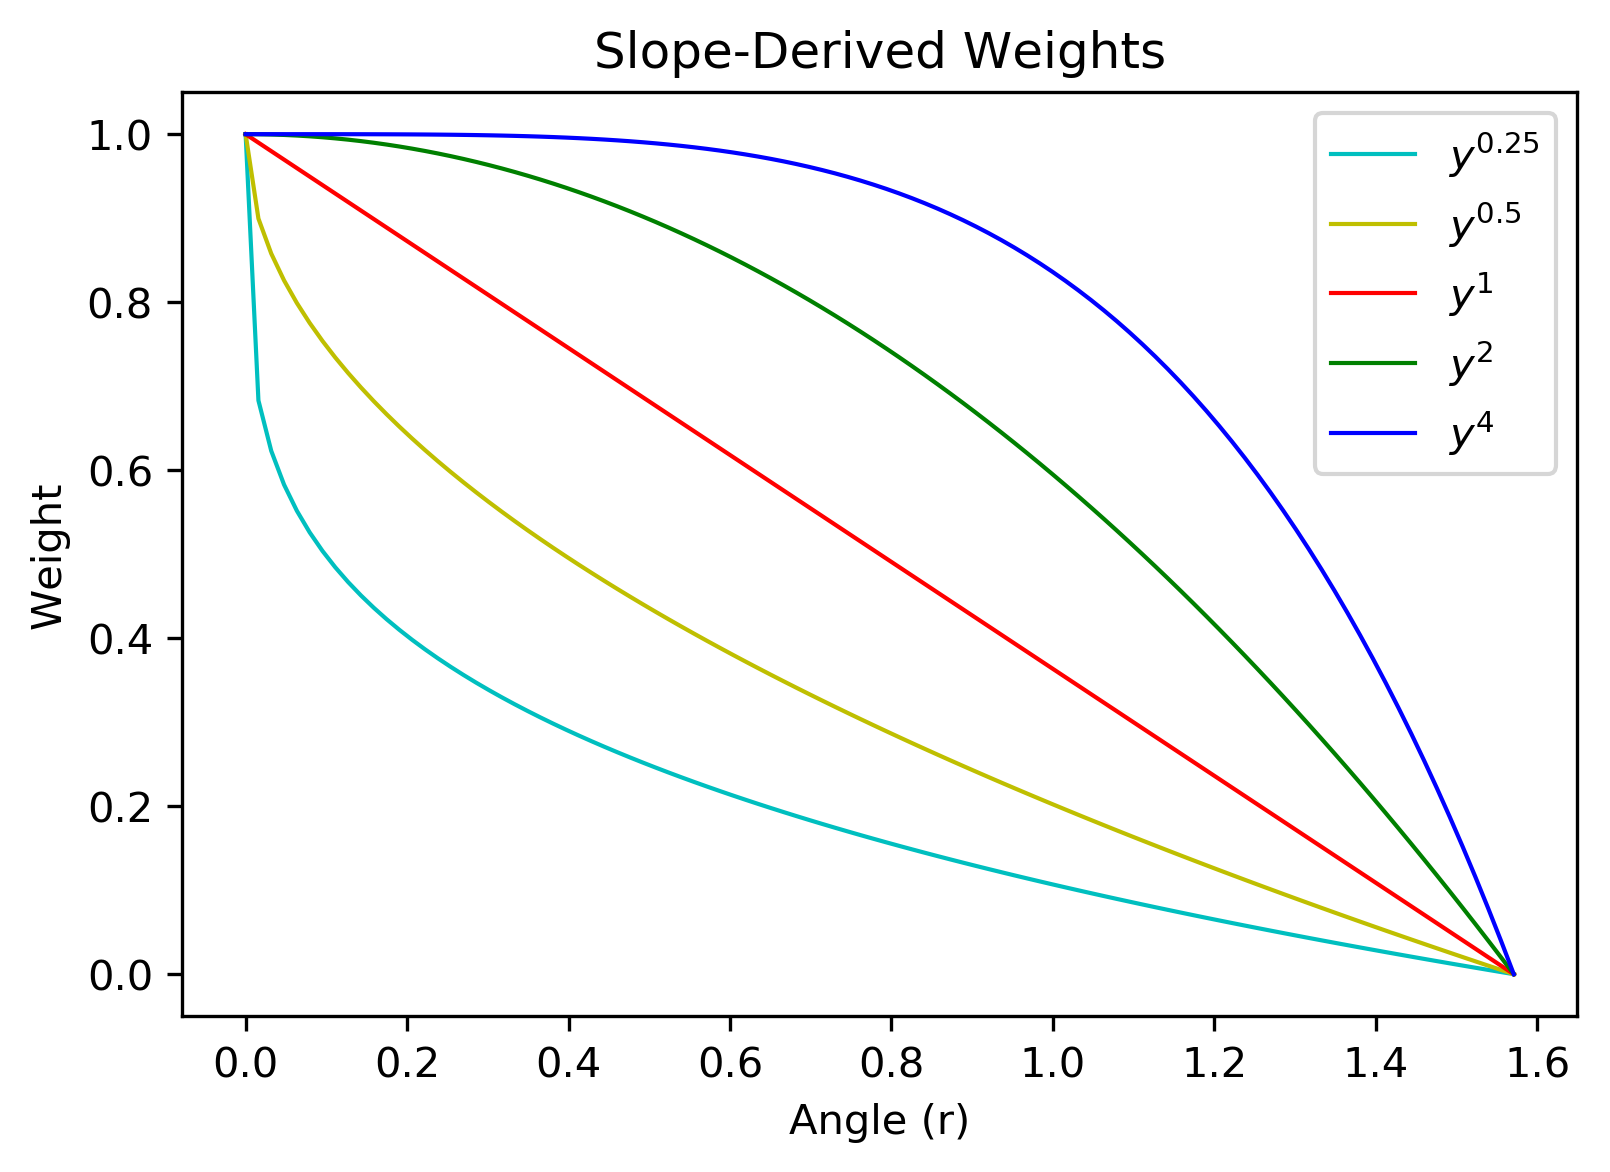
\includegraphics[width=1.0\linewidth]{tmp/slope_weights.pdf} 
\caption{Effect of the exponent on the slope- or angle-weight multiplier.}
\label{fig:slope_weight}
\end{figure}

\subsection{Point Clouds}

The point clouds were extracted from raw 3-dimensional LiDAR point clouds produced through the activities of the Hyperspectral-LiDAR Research group at the University of Victoria. Several sites were selected:

\subsubsection{Black Canyon, Thompson River, British Columbia}

This area (figure \ref{fig:thompson_map}) was surveyed by HLRG in August 2017 using a UAV and Velodyne VLP-16 LiDAR instrument. The terrain is mostly bare, except for the presence of small shrubs and trees. The average point density is $234.50points/m^2$ with a maximum of $759.00points/m^2$ and standard deviation of $110.32points/m^2$.

\begin{figure} %[htbp] % htbp stand for "here", "top", "bottom", "page"
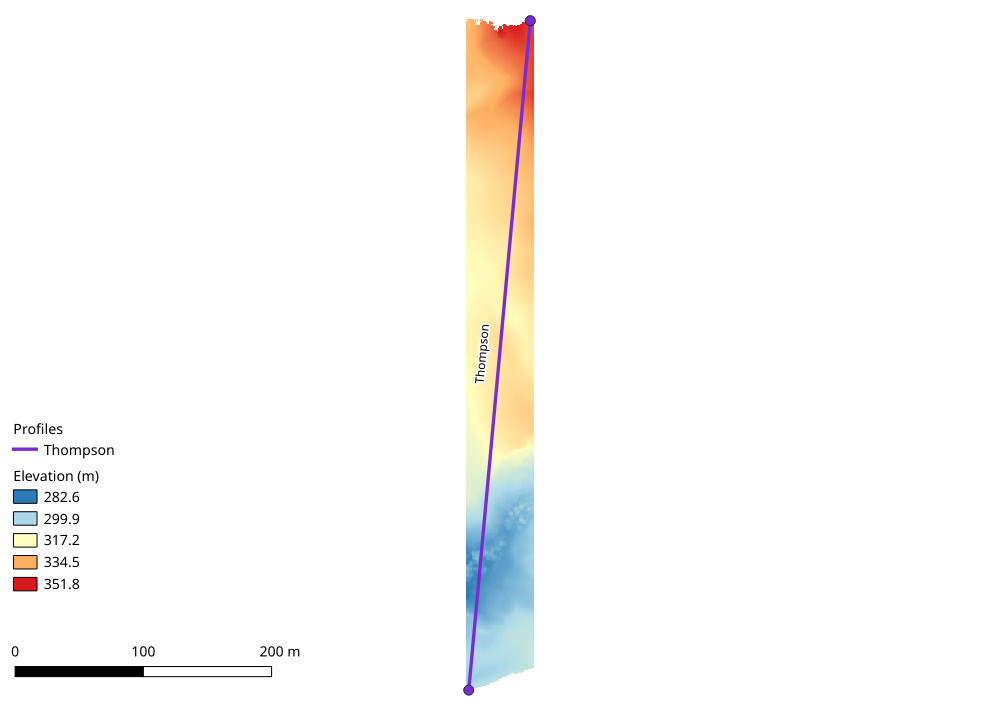
\includegraphics[width=1.0\linewidth]{tmp/thompson_map.pdf} 
\caption{Map of Thompson Canyon survey area showing extracted profile.}
\label{fig:thompson_map}
\end{figure}


\subsubsection{Bartier Brothers Winery, Okanagan, British Columbia}

This area (figure \ref{fig:bartier_map}) was surveyed by HLRG in August 2017 using a UAV and Velodyne VLP-16 LiDAR instrument. The terrain is covered with grape vines spaced at approximately $\SI{2}\m$. The average point density is $4999.73points/m^2$ with a maximum of $13612.00points/m^2$ and standard deviation of $2289.77points/m^2$. The profile passes over a wind generator approximately $\SI{5}\m$ in height.

\begin{figure} %[htbp] % htbp stand for "here", "top", "bottom", "page"
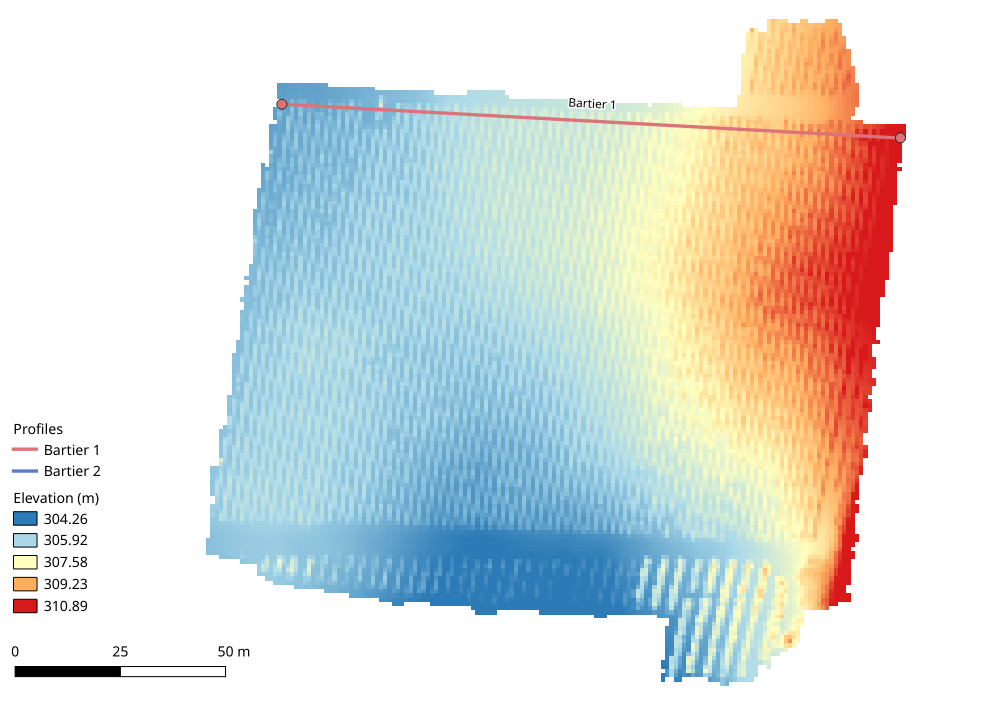
\includegraphics[width=1.0\linewidth]{tmp/bartier_map.pdf} 
\caption{Map of Bartier Brothers Winery survey area showing extracted profiles.}
\label{fig:bartier_map}
\end{figure}


\subsubsection{Mount Douglas and Blenkinsop Lake, Victoria, British Columbia}

This area was surveyed by HLRG using a manned aircraft and LiDAR instrument. In the Mount Douglas sector (figure \ref{fig:mt_doug_map}, northeast) the terrain is steep, covered with a mix of bare rock, mature second-growth Douglas fir and Garry Oak forests. In the Blenkinsop Lake area (figure \ref{fig:mt_doug_map}, center), there are fields of grass, second-growth Douglas fir and a small lake. Christmas Hill (figure \ref{fig:mt_doug_map}, southwest) is similar to Mount Douglas but smaller and surrounded by houses. The average point density is $5.62points/m^2$ with a maximum of $53.00points/m^2$ and standard deviation of $3.36points/m^2$.

\begin{figure} %[htbp] % htbp stand for "here", "top", "bottom", "page"
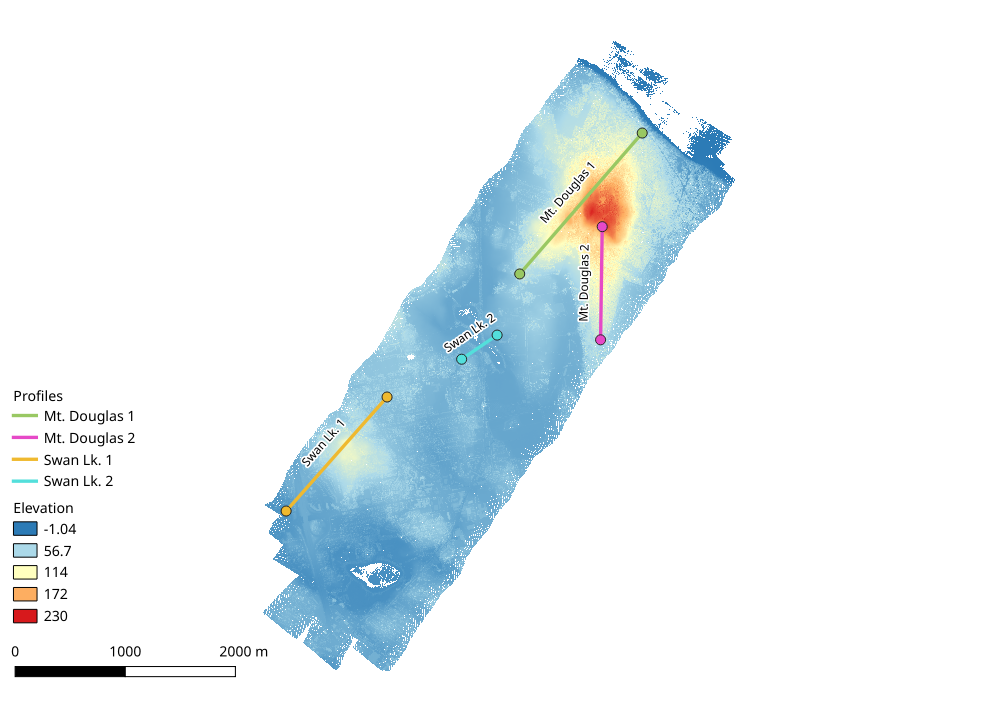
\includegraphics[width=1.0\linewidth]{tmp/mt_doug_map.pdf} 
\caption{Map of Mount Douglas, Blenkinsop Lake and Christmas Hill survey areas showing extracted profiles.}
\label{fig:mt_doug_map}
\end{figure}


\begin{figure} %[htbp] % htbp stand for "here", "top", "bottom", "page"
\begin{subfigure}[b]{\linewidth}
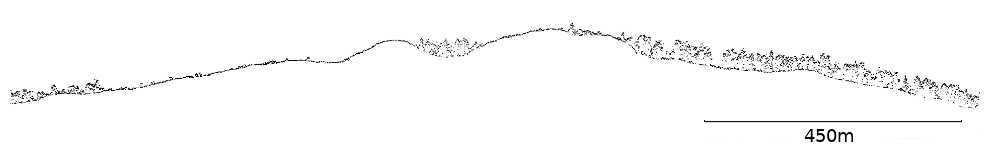
\includegraphics[width=1.0\linewidth]{tmp/mt_doug_1_profile.pdf} 
\caption{Mt. Douglas 1} \label{subfig:mt_doug_1}
\end{subfigure}
\begin{subfigure}[b]{\linewidth}
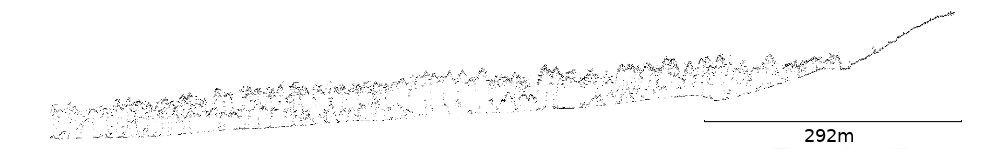
\includegraphics[width=1.0\linewidth]{tmp/mt_doug_2_profile.pdf} 
\caption{Mt. Douglas 2} \label{subfig:mt_doug_2}
\end{subfigure}
\end{figure}

\begin{figure}\ContinuedFloat
\begin{subfigure}[b]{\linewidth}
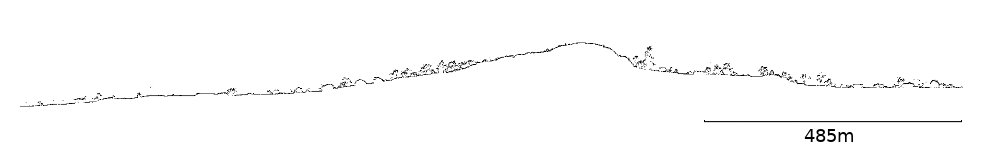
\includegraphics[width=1.0\linewidth]{tmp/swan_1_profile.pdf} 
\caption{Christmas Hill} \label{subfig:swan_1}
\end{subfigure}
\begin{subfigure}[b]{\linewidth}
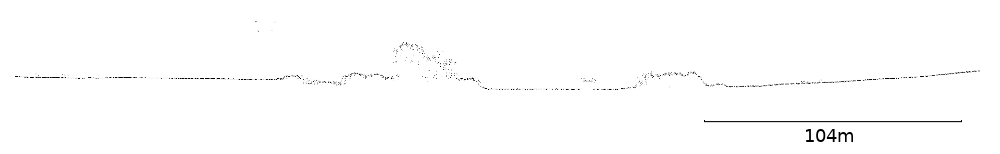
\includegraphics[width=1.0\linewidth]{tmp/swan_2_profile.pdf} 
\caption{Blenkinsop Lake} \label{subfig:swan_2}
\end{subfigure}
\end{figure}

\begin{figure}\ContinuedFloat
\begin{subfigure}[b]{\linewidth}
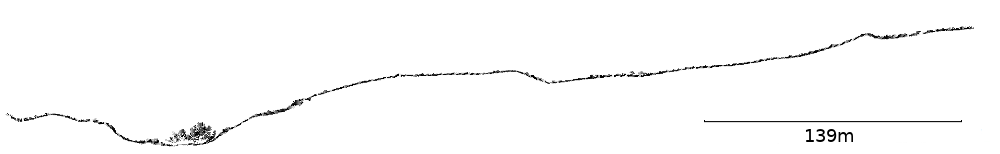
\includegraphics[width=1.0\linewidth]{tmp/thompson_profile.pdf} 
\caption{Black Canyon} \label{subfig:thompson}
\end{subfigure}
\begin{subfigure}[b]{\linewidth}
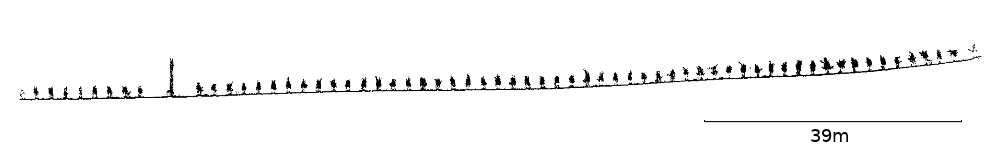
\includegraphics[width=1.0\linewidth]{tmp/bartier_1_profile.pdf} 
\caption{Bartier 1} \label{subfig:bartier_1}
\end{subfigure}
~
\caption{Point cloud sections. Note the difference in scale for each. The wind generator is clearly visible in (\ref{subfig:bartier_1}).}
\label{fig:profiles}
\end{figure}

\begin{table}
\caption{Point densities for each point cloud.}
\label{table:pt_density}
\begin{tabular}{l || r} 
Profile & Pts. / $m^2$ \\
\hline
Mt. Douglas 1  & 8.60 \\
Mt. Douglas 2  & 10.83 \\
Thompson       & 246.68 \\
Bartier 1      & 3724.11 \\
Christmas Hill & 7.99 \\
Blenkinsop Lk. & 6.69 \\
\end{tabular}
\end{table}


A scanning laser will ultimately be used for building the point cloud. At its maximum range of $\SI{100}\m$, and a scan angle of $\SI{5.7}\deg$, the swath is approximately $\SI{2}\m$. Therefore, a vertical hyperplane was intersected with each point cloud and the start and end points of each line, and any point which formed an acute angle with the start and end points was preserved. (The hyperplane's length is infinite; this strategy preserves only the points that lie between the endpoints.) The $x$-coordinate of each point was set to $0$, and the $y$-coordinate set to the Cartesian distance between it and the start point. The $z$-coordinates were unchanged. The resulting point clouds are shown in figure \ref{fig:profiles}. The point density of each profile is given in table \ref{table:pt_density}.

Each profile was subjected to the concave hull and spline algorithms in listing \ref{lst:concave_hull}, using a variety of inputs for the smoothing parameter $s$, the segment length $\alpha$, and an exponential weight for the vertex-weighting scheme. For each trial, several statistics were collected:

\begin{itemize}
\item The number of source points found above the spline.
\item The maximum distance from the spline to a point above it.
\item The minimum and maximum vertical velocity.
\item The minimum and maximum vertical acceleration.
\item The residual.
\end{itemize}

The points above the spline are used to determine whether the fit of the spline allows surface objects to project above the aircraft's trajectory, and by how much. If this distance is too large, the fit of the spline must be improved, or the flight altitude increased.

The minimum and maximum vertical velocity and acceleration serve to indicate whether the aircraft's propulsion system can produce enough force to ascend, and whether gravity is sufficient to descend, quickly enough to accomodate the trajectory. The velocity must also be within the flight controller's pre-set constraint.

The residual gives some indication of how well the trajectory fits the point cloud, though this is to an extent determined by the number of points, and thus upon $\alpha$.

\subsection{Aircraft}

The dynamic limits used for this study are those of the DJI Matrice 600 hexacopter. Some specifications for the vehicle are given in table \ref{table:djispecs}.

\begin{table}
\begin{center}
\begin{tabular}{ l r }
\hline
Vehicle weight (TB47S batteries) & $\SI{9.1}\kg$ \\ 
Vehicle weight (TB48S batteries) & $\SI{9.6}\kg$ \\
Maximum vehicle weight & $\SI{15.1}\kg$ \\
Maximum pitch angle & $\ang{25}$ \\
Maximum pitch velocity & $\SI{300}{\degree\per\second}$ \\
Maximum yaw velocity & $\SI{150}{\degree\per\second}$ \\
Maximum ascent velocity & $\SI{5}{\metre\per\second}$ \\
Maximum descent velocity & $\SI{3}{\metre\per\second}$ \\
Maximum horizontal velocity & $\SI{18}{\metre\per\second}$ \\
Maximum wind velocity & $\SI{8}{\metre\per\second}$ \\
Maximum thrust (per rotor) & $\SI{5100}{\g}$ \\
\hline
\end{tabular}
\end{center}
\caption{DJI Matrice 600 Specifications \cite{DJI2017}.}
\label{table:djispecs}
\end{table}

These constraints may not correspond to the absolute physical limits on vehicle performance, but they do provide a useful guide to the limits that may be imposed by the flight control API, and from these quantities, the dynamic limits of the platform (e.g., maximum thrust) may be inferred.

The nominal maximum thrust, $T_n$, generated by the DJI6100/DJI2170 motor/propeller combination is given as $\SI{5100}\g$ of pulling force per rotor \parencite{DJI2017}. The propulsive forces of the six rotors cannot be summed directly because their axes are not aligned. However, it is a simple matter to decompose the thrust vector of each into its $T_x$ and $T_z$, components ($T_z$ is vertical; $T_y$ is not required) and sum the $T_z$ components. The $T_x$ components can be ignored because, being radially opposed, they cancel out. Note that this is a gross oversimplification; there are other forces at play, such as torque and wind, but the object is to provide some guidence as to limits, not to produce an accurate dynamic model.

Measured from CAD drawings supplied by DJI \parencite{DJI2017}, each arm of the hexacopter is inclined upwards from horizontal by $8\deg$, or $0.139643114$ radians. The $T_z$ component is then,

\begin{equation}
\begin{split}
T_z &= sin(\theta) * T_n \\
T_z &= sin(0.139643114) * 5.1 \\
T_z &= 0.990265734 * 5.1 \\
T_z &\approx \SI{5.050}{\kg} % 5.050355244.
\end{split}
\end{equation}

This gives a total maximum thrust $T_{max}$ of,

\begin{equation}
\begin{split}
T_{max} &= 6 * T_z \\
T_{max} &\approx \SI{30.302}{\kg}.
\end{split}
\end{equation} 

We wish to represent the maximum available thrust as a force, $F_t$, in Newtons. Assuming a vertical orientation of the thrust vector and the acceleration of gravity as $g$, 

\begin{equation}
\begin{split}
F_t &= T_{max} * g \\
F_t &= T_{max} * 9.08665 \\
F_t &\approx \SI{297.162}{\N}
\end{split}
\end{equation}

At the maximum vehicle mass of $M_v = \SI{15.1}{\kg}$, this gives a maximum vertical linear acceleration of,

\begin{equation}
\begin{split}
a &= (F_t - F_g - F_d) / M_v \\
a &= (297.162397521 - (9.80665 * 15.1) - 0) / 15.1 \\
a &\approx \SI{9.873}{\m\s^{-2}}, %9.872978975
\end{split}
\end{equation}

where $F_g$ is the force of gravity and $F_d$ is the force of drag, which is zero, under the assumption that vertical accelerations begin during level flight.



\section{Results}

Because it was unknown how the smoothing spline would behave for each of the point cloud inputs, given the variety of point densities and relief variances, a brute-force strategy was applied to compute splines using a range of values for each parameter.

The alpha parameter was sampled from the set, $(1, 2, 5, 10, 25, 50)$. The smoothing parameter $s$ was calculated according to the documented suggestion (see equation \ref{eq:s_range}) and subjected to a multiplier: The minimum, maximum and median values from the range of $s$ were multiplied by a value sampled from a geometric sequence in the range $0.000001$ to $100$. For high-relief profiles, with a large variance in terrain elevations, a small smoothing parameter was required so as not to overwhelm the small weight values. For flatter surfaces, larger smoothing values would suffice. 

Weights were applied using the slope-weighting scheme and scaled using an exponent from the set $(0, 1, 2, 4)$. In the zero-exponent case, the weight would be a constant -- the inverse of the standard deviation in $z$.

There were 8640 individual trials on 6 datasets. The smoothing spline converges to a straight line when $s=0$ and an optimal  least-squares fit at some ``large'' value of $s$ (the algorithm performs a limited number of iterations, but generally converges with reasonable parameters). These conditions can be detected by duplicate output values for minimum and maximum acceleration and velocity, and the residual. The duplicates were filtered out, as were results which exceed the dynamic limits of the aircraft or which contain points too far above the trajectory, given a nominal altitude of $\SI{10}\m$. 

\begin{equation} \label{eq:filter_limits}
\begin{split}
v_{max} &< 5.0 \\
v_{min} &> -5.0 \\
a_{max} &< 9.873 \\
a_{min} &> -9.087 \\
p_{max} &< 10.0
\end{split}
\end{equation}

With the limits in (\ref{eq:filter_limits}), where $v$ is velocity, $a$ is acceleration, and $p$ is the height of points above the spline, the trial outputs were filtered using the query in listing \ref{lst:result_sql}, leaving 678 valid results (table \ref{table:arg_results}.)

\begin{listing}
\begin{minted}{sql}
with t as (
	select *, concat(vel_max, vel_min, acc_max, acc_min, residual) as key 
		from trials 
		where vel_max < 5 and vel_min > -5 and acc_max < 9.873 
			and acc_min > -9.807 and above_max < 10 
		order by filename, above_max, vel_max, 
			abs(vel_min), acc_max, abs(a308 & 50 & 1 & 4 & 0 & 0.848464 & 0.000872cc_max), residual
), u as (
	select filename, key, count(*) as ct 
		from t 
		group by key, filename
)
select t.filename, count(*) as results, max(alpha) as max_alpha, 
		min(alpha) as min_alpha, max(weight) as max_weight, 
		min(weight) as min_weight, max(smooth) as max_smooth, 
		min(smooth) as min_smooth 
	from t, u 
	where t.key=u.key and ct <= 1 
	group by t.filename;


\end{minted}
\caption{SQL query used for filtering trial results within predetermined limits and excluding converged results.}
\label{lst:result_sql}
\end{listing}



\begin{table}
\caption{Valid parameter ranges for smoothing spline trials.}
\label{table:arg_results}
\begin{tabular}{l | r || r | r | r | r | r | r} 
Profile & Count & Max. $\alpha$ & Min. $\alpha$ & Max. $w$ & Min. $w$ & Max. $s$ & Min. $s$ \\
\hline
Mt. Douglas 1  & 25  & 50 & 2 & 1 & 0 & 0.057574 & 0.003062 \\
Mt. Douglas 2  & 24  & 10 & 2 & 2 & 0 & 0.210198 & 0.001650 \\
Thompson       & 308 & 50 & 1 & 4 & 0 & 0.848464 & 0.000872 \\
Bartier 1      & 99  & 25 & 1 & 4 & 0 & 0.126134 & 0.000323 \\
Christmas Hill & 20  & 25 & 2 & 0 & 0 & 0.043681 & 0.002247 \\
Blenkinsop Lk. & 202 & 50 & 1 & 4 & 0 & 0.227740 & 0.000606\\
\end{tabular}
\end{table}

\begin{figure} %[htbp] % htbp stand for "here", "top", "bottom", "page"
\begin{subfigure}[b]{\linewidth}
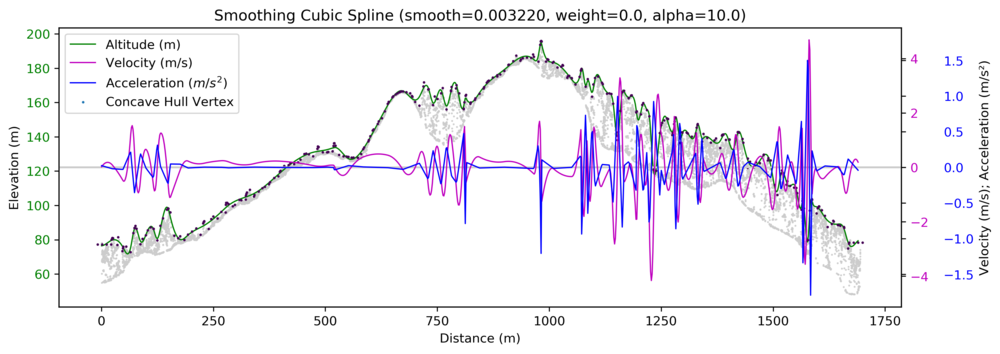
\includegraphics[width=1.0\linewidth]{tmp/mt_doug_1_2m_0_003220_10_00_0_000.pdf} 
\caption{Mt. Douglas 1} \label{subfig:mt_doug_1}
\end{subfigure}
\begin{subfigure}[b]{\linewidth}
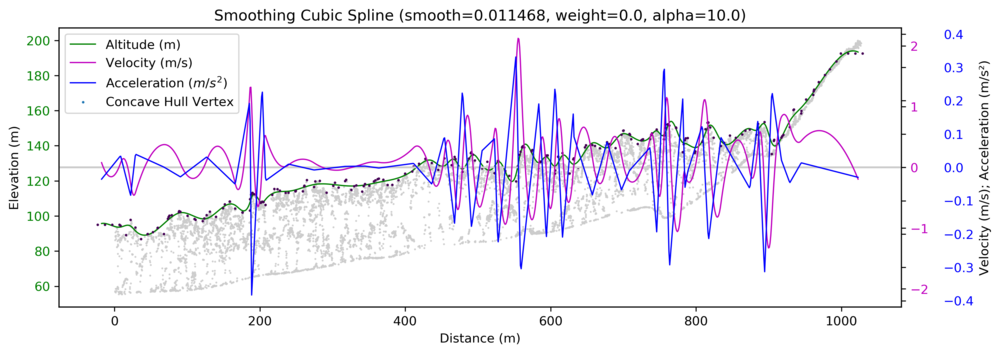
\includegraphics[width=1.0\linewidth]{tmp/mt_doug_2_2m_0_011468_10_00_0_000.pdf} 
\caption{Mt. Douglas 2} \label{subfig:mt_doug_2}
\end{subfigure}
\end{figure}

\begin{figure}\ContinuedFloat
\begin{subfigure}[b]{\linewidth}
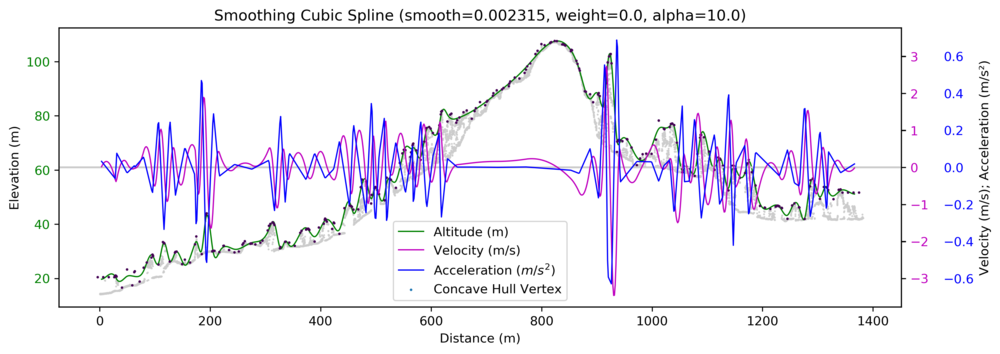
\includegraphics[width=1.0\linewidth]{tmp/swan_lk_1_2m_0_002315_10_00_0_000.pdf} 
\caption{Christmas Hill} \label{subfig:swan_1}
\end{subfigure}
\begin{subfigure}[b]{\linewidth}
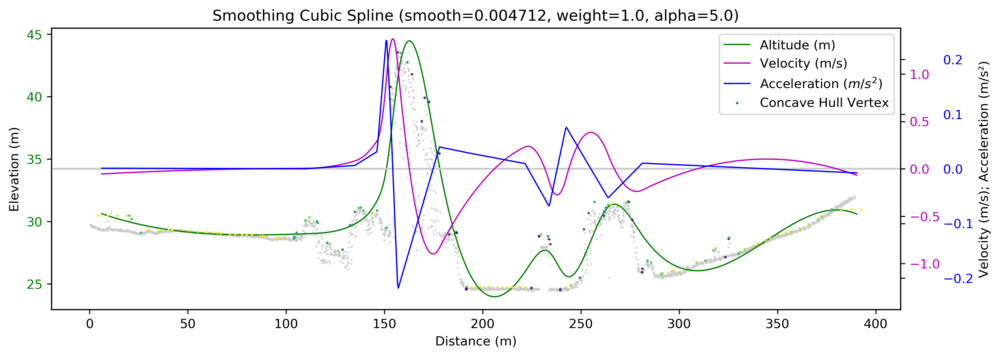
\includegraphics[width=1.0\linewidth]{tmp/swan_lk_2_2m_0_004712_5_00_1_000.pdf} 
\caption{Blenkinsop Lake} \label{subfig:swan_2}
\end{subfigure}
\end{figure}

\begin{figure}\ContinuedFloat
\begin{subfigure}[b]{\linewidth}
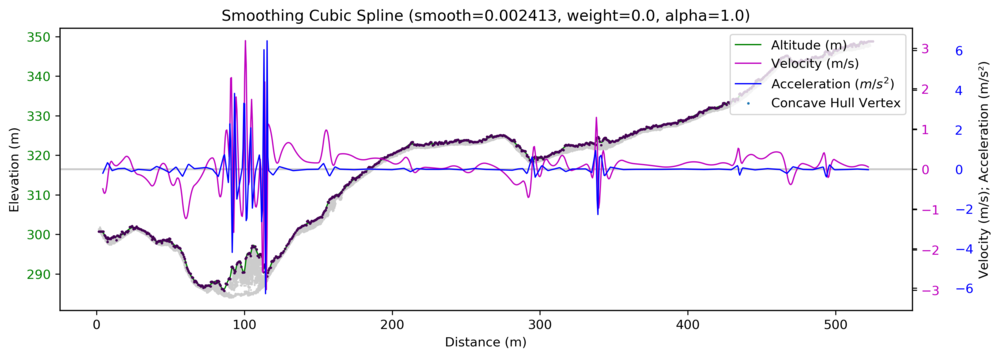
\includegraphics[width=1.0\linewidth]{tmp/nrcan_4_2m_0_002413_1_00_0_000.pdf} 
\caption{Black Canyon} \label{subfig:thompson}
\end{subfigure}
\begin{subfigure}[b]{\linewidth}
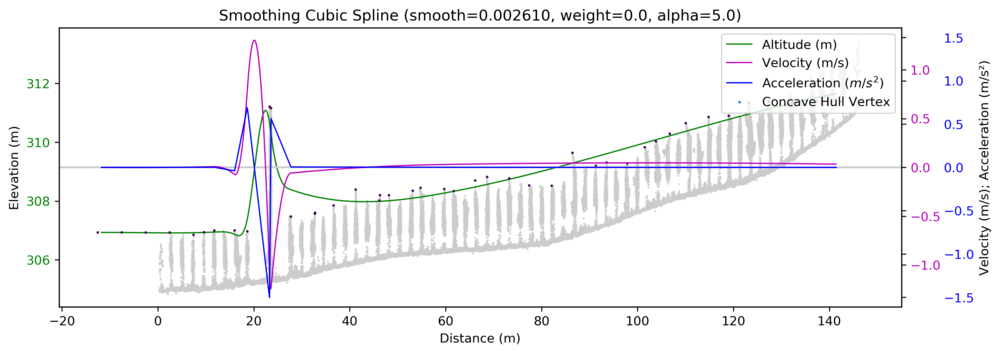
\includegraphics[width=1.0\linewidth]{tmp/VITI_D168_BART_sess12_v1_1_2m_0_002610_5_00_0_000.pdf} 
\caption{Bartier 1} \label{subfig:bartier_1}
\end{subfigure}
~
\caption{Trajectory, velocity and acceleration curves for each profile.}
\label{fig:profiles}
\end{figure}

Figure \ref{fig:profiles} shows a selection of smooth spline trajectories that obey the dynamic constraints of the aircraft and provide some reasonable fidelity to the imaged surface. It is apparent that there is a great deal of variability in terms of the length of a trajectory, the characteristics of the terrain relief, the high-frequency variation in the height of the surface, and the intentions of the surveyor. This project has demonstrated that it is possible to extract a trajectory from a point cloud, using cubic splines, which provides a means of quantifying the suitability of the trajectory for research and safety objectives.

However, there are some fatal flaws with the strategy. As the vehicle progresses along its trajectory, added data to the point cloud and re-computing the spline at intervals, the height of the spline is adjusted along its \emph{entire} length, including the section currently being navigated by the aircraft. This induces instantaneous ``jumps'' in the trajectory, which are not only deleterious in terms of data quality (and unquantifiable) but physically impossible for the aircraft to negotiate. 

\newpage

\printbibliography

\end{document}